% !TEX root = relative/or/absolute/path/to/root/file.tex
\documentclass[a4paper,12pt]{report}
\usepackage{graphicx}
\usepackage{amsmath}
\usepackage[utf8]{inputenc}
\usepackage[a4paper, margin=1in]{geometry}

\usepackage{setspace}   % For line spacing
\usepackage{parskip}    % For better paragraph spacing
\usepackage{titlesec}   % For customizing section titles



\title{Chess Engine\\
{\Large COMP4121}}
\author{Joshua Shim}
\date{November 2024}

\begin{document}
\maketitle
\chapter*{Abstract}

Chess is a simple game that is played on a $8 \times 8$ grid board, with 6 different types of pieces that each move differently. Intuitively it is a simple game. However due to the permutational complexity of this game, a large number of humans have dedicated their lives to chess and yet chess remains `unsolved'. Chess remains a highly theoretical board game where it remains subjective in many cases as to which move is the best.
\\\\
By the late 1980's computer chess programs had begun being competitive with top human players and 25 years later, the last known win against a top-performing computer by a human player was recorded in the Ponomariov vs Fritz game.
\\\\
Since then, as hardware and chess algorithmic theory have had noticeable improvements, the delta between human chess and computer chess programs have only increased.
\\\\
For the COMP4121 major project, I have chosen to make a chess engine from scratch. Coming from a pure computer science background with limited mathematical knowledge, I believe that the creation of a chess engine would allow me to actively learn about both the deterministic and randomised algorithms that allow chess engines to overcome the human brain. Hence I came up with the goal of creating a chess engine that would be able to beat the average human player.
\\\\
Initially, I had planned to create a chess engine that primarily utilised the \textit{Monte Carlo Tree Search} algorithm to search for the best moves. However due to the time constraints and the inability for me to feasibly tune the \textit{Monte Carlo Tree Search} using deep learning meant that a \textit{MCTS} chess engine would be significantly less impressive than a more standard chess engine that utilises the \textit{Min-Max Algorithm}.\newpage
The chess bot that I have created is named \textbf{COMP4121bot} and uses a \textit{Universal Chess Interface (UCI)} interface to communicate with the front-end. I have a Raspberry Pi 3 model B setup that runs the chess engine so that it exists as a bot on \textit{lichess.org} where it is available for play. I will keep it active on the website until 31/12/2024 and highly encourage you to play a game against it. Note that as it is running on lower end hardware, its performance is significantly lower than if it were to run on my desktop. The following game setup works but others may / may not be accepted by my bot:\\
Variant: Standard\\
Time Control: Real time\\
Minutes per side: 10\\
Increment in seconds: 3\\
Game Mode: Casual\\\\
% TODO: create a list of available game modes.
Play on this link (you may need to create an account):\\
https://lichess.org/@/COMP4121bot

\tableofcontents
\chapter{Board Representation}
A chess program requires an internal board representation to maintain the current locations of each piece and also additional information to identify whose turn it is to play, castling rights and whether an en passant move is possible. Furthermore, more advanced engines require additional data structures to keep track of previous moves in order to avoid \textit{threefold repetition} and the \textit{fifty-move rule}.
\section{Array}
The most intuitive board representation would be a $8 \times 8$ 2-dimensional array of 1 byte words. This board representation was the first design that had come to my mind. This design would also be quite space efficient, which was a big consideration for me as the \textit{Monte Carlo Tree Search} algorithm requires a tree data structure to be kept, with each \textit{node} containing a full board representation.\\\\
This particular board representation would allow for the whole board to be represented by \textbf{64 bytes} in total, as there are 64 slots of 1 byte each. As there are only 12 different types of pieces, only 4 bits are required to determine the colour of the piece and the type of the piece. This allows for the board to be represented with a lower byte count of \textbf{32 bytes} if we were to use 4 bit words for each cell of the array. Whereas this would be faster for systems that are optimised for 4 bit words, most modern systems and hardware is designed to handle 8-64 bit words, and therefore I would have chosen to take the larger sized array for higher speed if I had decided to use this design. Furthermore, more bits would be required to hold the additional information about the state of the game.\\\\
Despite the small size of the board representation, speed, which is arguably a greater concern when designing chess engines is much slower as opposed to using bitboards. This is because when we generate possible moves, it is necessary to loop through each cell, identify whether a piece exists within the cell, and if a piece does exist, then generate the possible destinations and create copies of the board for each destination that can be made for the selected piece. This must be done for each and every piece and unlike bitboards, we cannot use simple bitwise operations which are usually single instructions and requires much less overhead.

\section{Bitboards}
Bitboards are an array of 64-bit words that can represent the chess board. Because there are 2 colours and 6 different types of pieces, the usual bitboard representation consists of an array of 12 64-bit words, each \textit{bitboard} being a representation of the locations of their respective pieces. 1-bits inside the 64-bit bitboard represents a location where the piece exists, where the most significant bit represents $a8$ and the least significant bit represents $h1$. This results in a relatively dense board representation consisting of $12 \times 8 =$ \textbf{96} total bytes per board representation alongside additional bits for turns, castling rights and en passant.\\\\
Due to the balance of high performance and memory density of a bitboard representation, I decided to use bitboards as the internal board representation of my chess engine. The first 6 indices of my array are reserved for white pieces and the next 6 for the black pieces. They represent in order: pawns, knights, bishops, rooks, queens and the king. Aside from the 12 length array of 64-bit words, I have an additional 32 bit word to contain additional information about the game state as shown below.

\begin{figure}[ht]
    \centering
    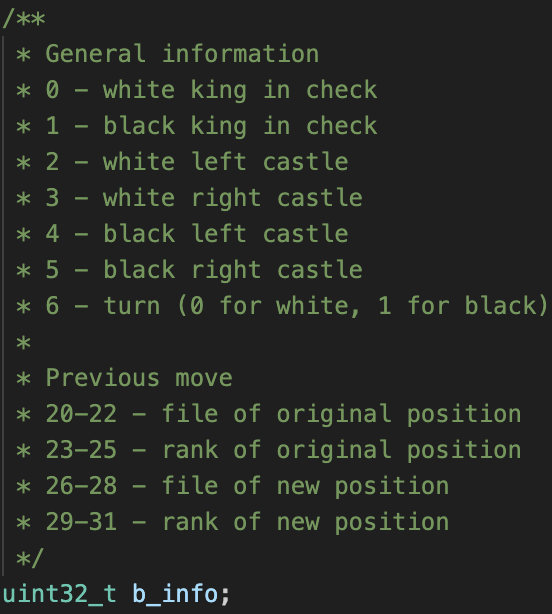
\includegraphics[width=0.8\textwidth]{images/sc1.png}
    % \caption{This is an example image.}
    % \label{fig:example-image}
\end{figure}
\chapter{Move Generation}
Chess engines aim to choose the best possible move that can be taken given the game state. Hence, chess engines typically generate all possible moves for the side whose turn it is. This provides the possibilities for the engine to pick moves from. Further moves are generated recursively from the newly generated moves in order to analyse how certain choices may lead to certain outcomes in the future, and to evaluate which move would be the best to take in the present. Here I will explain how moves are efficiently generated using bitboards as implemented in my chess engine.
\section{Precomputations and Optimisations}
A downside of the bitboard board representation is that it is computationally inefficient in finding whether a piece exists in any given square, whether that piece is black or white and which type of piece it is. Hence, an optimisation I have made is to precompute at the start of every move generation two 64-bit-masks, the first to indicate the squares that are occupied by the white pieces and the second for the black pieces. This is important for move generation as attacking moves must check that there is an enemy piece in the square that the piece is attacking and that there are no other pieces blocking it. Regular moves must also ensure that there are no pieces blocking their movements.\\\\
Furthermore, another optimisation that I have made was to generate all \textit{pseudo-legal} moves. Legal moves are moves that can be legally taken as per the rules of chess. The moves that my engine generates include illegal moves when the king is in check. Moves that don't uncheck the king are not removed in the list of moves returned by my move generation function. The logic behind this is that if the king is in check and an illegal move is made, either the MCTS or min-max algorithm, if correctly implemented would avoid taking that move as it would result in an automatic loss. If we were to generate moves to a depth of 2 in order to check for illegal moves as described, the time complexity of move generation would become $O(n^2)$ as opposed to $O(n)$, where $n$ is the largest number of possible moves. This has greater implications in the search function as the move evaluation function would be called recursively, compounding the increase in latency.\\\\
However, we cannot completely remove the need to check for whether a king is in check as the special move \textit{castling} requires the king to not be in check. Hence instead of checking for checks during move generation, I do so after a turn is finished and keep the info in the 32-bit word within my internal board representation. This step amortizes the latency generated by checking for checks.
\section{Special Moves}
There are two special moves that can be made in chess: Castling and En passant. Specific rules apply to these moves and therefore we must use additional bits allocated to our board representation.
\subsection{Castling}
Castling is a special move that involves the king and the rook. Castling requires both the king and the rook to be castled with to not have moved, the king to not be in check and there to not exist pieces between the king and the rook. Hence for each side, we must reserve two bits each to indicate whether a respective rook has moved or not and we can set both bits to not allow castling if the king has moved. After each turn, we check for checks and set a bit for if the king is in check. By reading this bit, we can check whether the king is in check to decide whether to allow castling or not.
\subsection{En Passant}
En Passant is a special move that translates to \textit{``on passing"} and involves the pawns. If playing as white and one of your pawns is on rank 5 and black does a \textit{double push} move with one of its pawns on an adjacent file, you may take the recently moved pawn as if it had done a \textit{single push}. The same applies for black on rank 4. Hence it is necessary to keep track of the most recently moved piece as En Passant is only a possible move if the enemy pawn had passed your pawn in the most recent move. My solution to this problem was to keep track of the new position and old position of the most recently moved piece. As there are a total of 8 ranks and files, $3\times 2\times 2 = 12$ bits in total were required to store the old position's rank and file and the new position's rank and file.
\section{Non-Sliding Moves}
Non-Sliding moves in chess are moves that have limited range but can happen regardless of enemy obstruction. This includes moves from pawns, knights and kings. Bitboards allow for very efficient non-sliding move generation as we could generate a non-sliding move for every piece in one cpu instruction then mask out the unavailiable moves through another instruction. For example, we could create every possible \textit{double push} for all the white pawns by left-shifting the white pawn bitboard by 16 bits. Then we could use two \&= operations to mask out possible destinations where the pieces are obstructed by either enemy or friendly pieces.\\\\
After generating all of the possible destinations, I then loop through each bit in the newly created destination bitboard by selecting the least significant 1-bit and then creating a copy of the original board where the the piece moves to the new destination and push the new board/move to the list of generated moves. The selection of the least significant bit is done using the NEGATION operator, then then and operator AND. This works as the negative of a number is represented by the two's complement, where the negation is the NOT of the number + 1. Hence the least significant bit is preserved whilst all the higher significance bits are masked out. After the copy is created and pushed into the list, an xor operation \textit{\^} with the \textit{destinations} bitboard allows me to remove the used destination. A similar process is used to generate the new boards for sliding moves.
\section{Sliding Moves}
Sliding moves in chess are moves that have unlimited range until obstructed by another piece or by the border of the board. Examples include the rook/queen's horizontal and vertical movements and the bishop/queen's diagonal movements. I implemented sliding moves in my engine by hardcoding each possible direction that a piece could move, appropriately shifting the previous location and if not obstructed using the OR operation to add to a \textit{destinations} bitboard. This is repeated until the direction is obstructed by a friendly piece. if obstructed by an enemy piece, the OR operation is done for the destination bitboard but the loop is broken as to not generate moves where the enemy piece is passed.
\chapter{Move Evaluation}
The move evaluation function is one of the most important aspects of a chess engine as it is what essentially determines the move that is to be selected by the chess engine. With perfect heuristics, the search function loses relevancy as it would be possible to determine the best move/position through the move evaluation alone.
\section{Piece Value}
My original move evaluation function began as a simple addition subtraction function that attributed points to each type of piece, multiplied the number of existing pieces by these points and took the sum of these points as the total points for each side. Then the advantage could be calculated through the difference between the sum of each side. \[
\text{white\_advantage} = wp \cdot 100 + wn \cdot 300 + wb \cdot 325 + wr \cdot 500 + wq \cdot 900 \\
- (bp \cdot 100 + bn \cdot 300 + bb \cdot 325 + br \cdot 500 + bq \cdot 900)
\]
Despite being a rather simple evaluation function, it is possible to create a relatively strong chess engine using such a simple evaluation function. An advantage of this evaluation function is that it is very fast to compute and may allow for more time and potentially deeper searches. Conversly, this approach fails to be effective at the start of the game as simple searchs usually do not allow for nuanced positioning and piece development that may aid the engine later on. A similar issue is faced during the endgame for similar reasons. However it is possible to complement the evaluation function and move generation to avoid these problems. For example a trie database of Grandmaster Chess games could be relied on at the start to allow for the chess engine to play more naturally.
\section{Positional Value}
A more complicated and nuanced approach is to consider the value that is to be had from occupying certain positions on the chess board. For example a knight in the centre of the board is arguably more valuable than a knight on the edge or corner of the board as it allows for more options for the knight and furthermore allows the knight to control more squares. Likewise pawns that are closer to being promoted are more valuable than pawns that are far from being promoted as these pawns have to possibility to become the most valuable piece in the game.\\\\
Positional values are especially more important in endgames where computer programs may not be able to plan ahead for checkmates with limited pieces. The Manhattan Distance \[d = \sum_{i = 1}^{n}|x_i - y_i|\]is especially useful as we may use it to give bonus advantage points when the enemy king is nearer to the corners of the board for easier checkmates.\\\\
My final implementation used the both the piece value alongside the positional values with the addition of the manhattan distance to aid in endgames. Due to a lack of time and hardware required for tuning for good positional value heatmaps, credit for the heatmaps go to Romain Goussault's Deepov Chess Engine: \textit{https://github.com/RomainGoussault/Deepov.git}
\chapter{Monte Carlo Tree Search}
\textit{MCTS} is a randomised algorithm that uses the \textit{Monte Carlo Method} to search game-trees. Initially developed for creating engins for Go, this algorithm can also be used to create chess engines. However, due to the arguably higher complexity of chess, it is more difficult to create a \textit{MCTS} chess engine, though examples such as AlphaZero and Leela exist to prove that \textit{MCTS} engines are competitive with the more traditional min-max engines. 
\textit{MCTS} runs in a loop, each iteration involving travelling down the tree. Traditionally, the most travelled branch is chosen by the engine. Each iteration involves the four steps that are outlined below:
\section{Selection}
We start from the root of the tree, which regarding chess engines is the current state of the board. In my (unused) implementation of MCTS, I had created a wrapper class named ``MCnode'' which has a aggregation relationship with its parent node and an composition relation with its child nodes. In C++ code this is represented through a optional raw pointer and a list of unique pointers respectively. This allows for a correct tree representation, the root node having no parent (hence the optional) and each node having a list of children which are owned by the parent. Hence if the parent is deleted, due to C++ 20 smart pointers, the children are also deleted.\\\\
Given this tree, the selection process of a \textit{MCTS} is a process that is repeated until a leaf node (node without any children or in this case a node with an empty children list) is reached. At a particular node, which child will be selected is determined by the \textit{UCT} or Upper Confidence Bound 1 Applied to Trees. This is calculated given the following formula \[\frac{w_i}{n_i} + c\sqrt{\frac{\ln{N_i}}{n_i}}\] where \begin{itemize}
    \item $w_i$ is the number of wins for the considered child node after $i$ iterations
    \item $n_i$ is the number of simulations for the considered child node $i$ iterations
    \item $N_i$ is the number of simulations after the $i^th$ move for the parent of the considered node
    \item $c$ is the exploration parameter which is a constant and may be tweaked to optimise the behavior of the engine
\end{itemize}
This function ensures the following:
\begin{itemize}
    \item Undiscovered nodes are always discovered before already discovered nodes as the \textit{UCT} of undiscovered nodes is infinity (divided by zero)
    \item Nodes when visited multiple times are less likely to be visited again unless the number of wins also increase
\end{itemize}
This ensures that undiscovered nodes are visited whilst also ensuring that nodes that often win are visited the most.
\section{Expansion}
When a leaf node is selected in the \textit{Selection} process, the expansion process begins. This process involves generating children for the leaf node. In Chess it is usually beneficial to generate all possible moves as the children and after the child nodes are generated one of these child nodes are chosen randomly.
\section{Simulation}
In simulation, we use the chosen node in the previous process (\textit{Expansion}) to do a random playout. If the engine's side wins then we increment the $w_i$ for the chosen node. However, due to chess' high branching factor from the large number of moves that can be played, such a purely random playout is usually not a reliable method to determine whether a win or loss can be recorded. Hence I decided to replace this random simulation with a min-max algorithm score computation with a depth of 3. I chose this method as I believed that this would provide a more accurate determination of whether there is an advantage to be gained by pursuing this branch, whilst taking an insignificant amount of computational time, allowing for more iterations to be run every round.
\section{Backpropagation}
Backpropagation is the last step of the \textit{MCTS} algorithm. This process involves recursively backtracking and updating the $n_i$ and $w_i$ figures as necessary from the result of the previous step. This can be done by traversing through the parent node until a std::nullopt is reached in my code.
\section{Summary}
Despite creating a ``functional'' MCTS algorithm for my chess engine, I ultimately chose not to use the MCTS algorithm for my final project, but instead to keep the code for future extensions. This is as I had lacked the time and resources (gpu) necessary to create a MCTS chess engine strong enough to defeat an average chess player (me) as MCTS chess engines are inevitably more complicated than traditional min-max engines. This is as MCTS engines require strong chess heuristics and detailed tuning preferably through deep learning to optimise the UCT calculation and simulation process.
\chapter{Min-Max Algorithm}
The min-max algorithm is the most commonly used algorithm when implementing chess engines. As opposed to MCTS, it has the advantage of being simpler to implement, computationally faster (when optimsed) and requires less tuning. The min-max algorithm begins as an exhaustive search, exploring each and every possibility up to a certain depth and assigning scores for all of the leaves in the hypothetical tree using the evaluation function. The min-max algorithm takes the lowest score of the ``children'' for the parents to account for the worst case scenario. Then, in the highest layer, the best of the worst scores is taken as the move chosen by the engine. A minor improvement that is made to the min-max algorithm is the ``negamax'' algorithm, which uses the fact that chess is a two sided game and as advantages are calculated for the current side, the best score of the previous layer can be taken as a negative to form the worst possible score of the current layer. This allows the algorithm to become fully recursive and therefore easier to read. Unlike the MCTS algorithm, a data structure is not required to store the possible movements as each possible move or board state is only visited once. Furthermore, this algorithm is easier to implement using multithreading as there are no problems involving concurrent data structure alterations. Hence in my implementation of the min-max algorithm, I multithread the computation of the first depth of the min-max algorithm. Remembering Amdahl's Law: \[S = \frac{1}{1 - p + \frac{p}{n}}\] $p$ in our case is almost 1 due to the fact that the branching factor in chess not varying greatly due to each branch originating from the same source and being of the same depth. 
\section{Alpha-Beta Pruning}
The min-max algorithm is an exponential-time algorithm with a time complexity of $O(b^d)$, where $b$ is the branching factor and $d$ is the depth of search. This is as for every possible move, every possible move of each possible move must be visited in the min-max algorithm. Hence without any optimisations, a high depth of search is infeasible as chess is usually played with time control. As depth is quite important when creating a strong chess engine, this is an important problem to fix.\\\\
The most common solution to this problem is \textit{alpha-beta pruning}. This is an addition to the min-max algorithm which keeps the \textit{alpha} (representing the best value that the maximising player can currently guarantee) and the \textit{beta} (representing the best value that the minimising player can currently guarantee). This allows us to use a conditional to ``prune'' branches that are worse than the current \textit{alpha}, drastically reducing computation time. As we traverse into a lower depth, we swap and negate the \textit{alpha} and \textit{beta} values as the turn and hence perspective changes by virtue of the ``negamax'' algorithm.\\\\
What this achieves is the ``pruning'' of branches that are unrealistic because the opponent would not choose them because they are worse than the opponent's best possible choice and also branches that are bad than our best choice. Whilst the time complexity of the worst case remains the same $O(b^d)$ as if the worst moves are explored first in ascending order no branches will be pruned, the time complexities of the average and best cases become much better becoming $O(b^{\frac{3d}{4}})$ and $O(b^{\frac{d}{2}})$ respectively. 
\section{Move Ordering}
In order to ensure that the best case time complexity of the improved min-max algorithm is achieved, it is imperative that the best moves are search first so that the worse moves can be pruned. If a bad move is searched before a better move is found, then the bad move would be fully searched without being pruned. using the heuristic that moves that attack pieces and moves that check pieces, chess engines often order their moves such that moves that check the king or attack another piece is moved to the front of the list. In more advanced chess engines, more advanced heuristics can be used for better move ordering, but my implementation followed the simpler approach of placing the attacking moves to the front. This required me to replace the std::vector that I was originally using with the std::deque (double ended queue) for faster at front insertions. Despite a std::list being identical in terms of time complexity, the principle of spatial locality means that the deque is faster as the C++ deque implementation is largely contiguous in memory whereas the list can be scattered throughout memory using indirection to access the next element. Hence elements in the deque are more likely to be in cache resulting in faster computations.
\chapter{Possible Improvements}
Above, I have given a brief summary of the thought processes and construction of my chess engine. In retrospect, creating the chess engine tested my software engineering skills more than my algorithmic knowledge and the result was exactly as I had originally planned, a chess engine that was better than what I believed an average chess player was (me). However there is a lot of room for improvements aside from the bugfixing (discussed in the next chapter) that I could not due to time constraints and scope implement. However I have done research about the theory and plan to implement these concepts either as an extension of this chess engine or if I decide to make a chess engine that runs on cleaner code. Here is a list of improvements that I had been planning to make to the chess engine in the future: 
\section{Quiescence Search}
One of the weaknesses of chess engines that use the min-max algorithm is that we cannot use a high depth due to the NP nature of the algorithm. For example, my chess engine can only feasibly operate on depth 6 on a ryzen 5 7600x cpu, with multithreading enabled. Even with further optimisations, as the time complexity is exponential, going beyond depth 7 would be unattainable. Hence, it is possible for a human to create a attack cycle that is greater than 7 moves long to trick the computer into playing bad moves. To prevent this and to also allow the computers to devise similar such tactics, we can implement something called \textit{Quiescence Search}. Quiescence search is essentially extending the min-max algorithm until the game state is quiet, by considering only moves that take other pieces or check a king until the game state becomes quiet (no such moves can be made). This allows the chess engine to meaningfully deepen the search without incurring too much of a performance penalty.
\section{Zobrist Hashing}
If one comes from a competitive programming background and thinks about how to increase the computational speed of a program, it is likely that they would think about dynamic programming. More specifically how we can cache results that have already computed to reduce the computational latency. A similar concept exists in chess programming where one creates a transposition table to store already discovered moves. One of the most popular ways to do this is through \textit{Zobrist Hashing}, which is a process that essentially converts game states into 64-bit word keys that correspond to values that usually contain the best move from that particular position. This allows for a $O(1)$ lookup for the best move if the same game state is reached, and by keeping a counter it becomes trivial to implement a system that prevents the \textit{threefold repetition rule} by keeping count of how many times the same state is reached.\\\\
Zobrist Hashing is an instance of tabulation hashing which is a method of creating universal families of hash functions through combining table lookup with xor operations. We convert the current chess board into a 64-bit word which becomes the key to be tabulation hashed. The process of tabulation hashing is as follows:
\begin{enumerate}
    \item We choose a $p = 64$ where $p$ is the number of bits in the key
    \item We choose a $q$ which is the number of bits to be in the output
    \item Choose a block size $r \leq p$, where a small $r$ uses less memory but is faster and vice versa
    \item $t = \lceil \frac{p}{r}\rceil$, which becomes the number of blocks that are required to form a key
    \item Create a 2D array $T[2^r][t]$, which is filled with random $q$-bit words
    \item To hash any key $k$, we split $k$ into $r$ bits each then the hash $h(k)$ is:
    \item $h(k) = T[0][k_0] \oplus T[1][k_1] \oplus \dots \oplus T[t - 1][k_{t - 1}]$

\end{enumerate}
\section{Start-Game Database}
Lastly, in order to address one of the major weaknesses of chess engines in general - that they cannot perform well in the start game due to their inability to look far enough into the game to properly develop pieces strategically as a human player would using chess theory, a start game database can be implemented using the many online databases of elite chess games on the internet. The idea would be to compile a set of these elite chess games as a trie data structure and until a certain number of moves, the engine follows the trie randomly to follow how human players would develop their pieces at the beginning. This would allow for the chess engine to have a fast earlygame, thus saving time for the future mid-game where the chess engine can dominate due to the chaotic nature of mid-games in chess.
\chapter{Known Bugs}
Here is a list of known bugs that I have been either reluctant to fix due to their insignificance regarding scope of the project or unable to fix.
\section{Triple Repetition}
In the late game, due to the fact that my chess engine does not cache recently made moves, triple repetition stalemates are a regular occurance. This occurs as the chess engine determines that a certain move is the best in a certain game state and as the min-max algorithm is deterministic, in a repetitive board state occurance, the same move will always be chosen by my chess engine.
\section{Stalemate}
In the late game, when my chess engine has a sizeable advantage, my chess engine sometimes actively pursues a stalemate where the enemy cannot make a legal move as it computes that this state is equal to a win. This is a product of my pseudo-legal move generation where moves where the king moves into check are also considered, meaning that such a stalemate allows for my engine to anticipate the taking of the enemy king in the move after the stalemate and considers such a state as equivalent to a win.
\section{Inevitable Loss Resignation}
When my chess engine is about to be checkmated and is currently in check, it sometimes attempts an illegal move. This is also a product of the pseudo-legal move generation as it believes that all moves are equally bad (-inf) and chooses a random move. Lichess reads such a move as a resignation but I have not fixed this bug as it does not affect the performance of the chess engine as it only resigns in situations where it is inevitably going to lose.
\section{Move Evaluation Double Error}
Late into the game, in some games, the evaluation function becomes corrupted and exorbitantly large numbers are attributed to some moves by the evaluation function. I am unaware of why this occurs and have not yet found out. However, it is not a very common occurance and my chess engine remains largely functional.

\end{document}